\documentclass[1p]{elsarticle_modified}
%\bibliographystyle{elsarticle-num}

%\usepackage[colorlinks]{hyperref}
%\usepackage{abbrmath_seonhwa} %\Abb, \Ascr, \Acal ,\Abf, \Afrak
\usepackage{amsfonts}
\usepackage{amssymb}
\usepackage{amsmath}
\usepackage{amsthm}
\usepackage{scalefnt}
\usepackage{amsbsy}
\usepackage{kotex}
\usepackage{caption}
\usepackage{subfig}
\usepackage{color}
\usepackage{graphicx}
\usepackage{xcolor} %% white, black, red, green, blue, cyan, magenta, yellow
\usepackage{float}
\usepackage{setspace}
\usepackage{hyperref}

\usepackage{tikz}
\usetikzlibrary{arrows}

\usepackage{multirow}
\usepackage{array} % fixed length table
\usepackage{hhline}

%%%%%%%%%%%%%%%%%%%%%
\makeatletter
\renewcommand*\env@matrix[1][\arraystretch]{%
	\edef\arraystretch{#1}%
	\hskip -\arraycolsep
	\let\@ifnextchar\new@ifnextchar
	\array{*\c@MaxMatrixCols c}}
\makeatother %https://tex.stackexchange.com/questions/14071/how-can-i-increase-the-line-spacing-in-a-matrix
%%%%%%%%%%%%%%%

\usepackage[normalem]{ulem}

\newcommand{\msout}[1]{\ifmmode\text{\sout{\ensuremath{#1}}}\else\sout{#1}\fi}
%SOURCE: \msout is \stkout macro in https://tex.stackexchange.com/questions/20609/strikeout-in-math-mode

\newcommand{\cancel}[1]{
	\ifmmode
	{\color{red}\msout{#1}}
	\else
	{\color{red}\sout{#1}}
	\fi
}

\newcommand{\add}[1]{
	{\color{blue}\uwave{#1}}
}

\newcommand{\replace}[2]{
	\ifmmode
	{\color{red}\msout{#1}}{\color{blue}\uwave{#2}}
	\else
	{\color{red}\sout{#1}}{\color{blue}\uwave{#2}}
	\fi
}

\newcommand{\Sol}{\mathcal{S}} %segment
\newcommand{\D}{D} %diagram
\newcommand{\A}{\mathcal{A}} %arc


%%%%%%%%%%%%%%%%%%%%%%%%%%%%%5 test

\def\sl{\operatorname{\textup{SL}}(2,\Cbb)}
\def\psl{\operatorname{\textup{PSL}}(2,\Cbb)}
\def\quan{\mkern 1mu \triangleright \mkern 1mu}

\theoremstyle{definition}
\newtheorem{thm}{Theorem}[section]
\newtheorem{prop}[thm]{Proposition}
\newtheorem{lem}[thm]{Lemma}
\newtheorem{ques}[thm]{Question}
\newtheorem{cor}[thm]{Corollary}
\newtheorem{defn}[thm]{Definition}
\newtheorem{exam}[thm]{Example}
\newtheorem{rmk}[thm]{Remark}
\newtheorem{alg}[thm]{Algorithm}

\newcommand{\I}{\sqrt{-1}}
\begin{document}

%\begin{frontmatter}
%
%\title{Boundary parabolic representations of knots up to 8 crossings}
%
%%% Group authors per affiliation:
%\author{Yunhi Cho} 
%\address{Department of Mathematics, University of Seoul, Seoul, Korea}
%\ead{yhcho@uos.ac.kr}
%
%
%\author{Seonhwa Kim} %\fnref{s_kim}}
%\address{Center for Geometry and Physics, Institute for Basic Science, Pohang, 37673, Korea}
%\ead{ryeona17@ibs.re.kr}
%
%\author{Hyuk Kim}
%\address{Department of Mathematical Sciences, Seoul National University, Seoul 08826, Korea}
%\ead{hyukkim@snu.ac.kr}
%
%\author{Seokbeom Yoon}
%\address{Department of Mathematical Sciences, Seoul National University, Seoul, 08826,  Korea}
%\ead{sbyoon15@snu.ac.kr}
%
%\begin{abstract}
%We find all boundary parabolic representation of knots up to 8 crossings.
%
%\end{abstract}
%\begin{keyword}
%    \MSC[2010] 57M25 
%\end{keyword}
%
%\end{frontmatter}

%\linenumbers
%\tableofcontents
%
\newcommand\colored[1]{\textcolor{white}{\rule[-0.35ex]{0.8em}{1.4ex}}\kern-0.8em\color{red} #1}%
%\newcommand\colored[1]{\textcolor{white}{ #1}\kern-2.17ex	\textcolor{white}{ #1}\kern-1.81ex	\textcolor{white}{ #1}\kern-2.15ex\color{red}#1	}

{\Large $\underline{11n_{162}~(K11n_{162})}$}

\setlength{\tabcolsep}{10pt}
\renewcommand{\arraystretch}{1.6}
\vspace{1cm}\begin{tabular}{m{100pt}>{\centering\arraybackslash}m{274pt}}
\multirow{5}{120pt}{
	\centering
	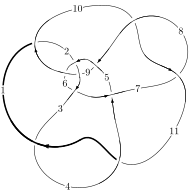
\includegraphics[width=112pt]{../../../GIT/diagram.site/Diagrams/png/778_11n_162.png}\\
\ \ \ A knot diagram\footnotemark}&
\allowdisplaybreaks
\textbf{Linearized knot diagam} \\
\cline{2-2}
 &
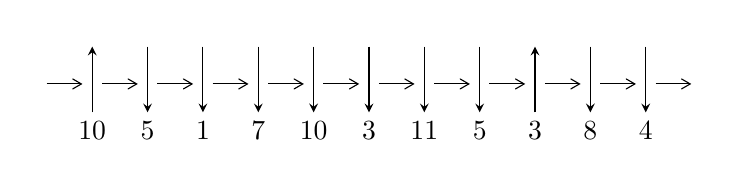
\begin{tikzpicture}[x=20pt, y=17pt]
	% nodes
	\node (C0) at (0, 0) {};
	\node (C1) at (1, 0) {};
	\node (C1U) at (1, +1) {};
	\node (C1D) at (1, -1) {10};

	\node (C2) at (2, 0) {};
	\node (C2U) at (2, +1) {};
	\node (C2D) at (2, -1) {5};

	\node (C3) at (3, 0) {};
	\node (C3U) at (3, +1) {};
	\node (C3D) at (3, -1) {1};

	\node (C4) at (4, 0) {};
	\node (C4U) at (4, +1) {};
	\node (C4D) at (4, -1) {7};

	\node (C5) at (5, 0) {};
	\node (C5U) at (5, +1) {};
	\node (C5D) at (5, -1) {10};

	\node (C6) at (6, 0) {};
	\node (C6U) at (6, +1) {};
	\node (C6D) at (6, -1) {3};

	\node (C7) at (7, 0) {};
	\node (C7U) at (7, +1) {};
	\node (C7D) at (7, -1) {11};

	\node (C8) at (8, 0) {};
	\node (C8U) at (8, +1) {};
	\node (C8D) at (8, -1) {5};

	\node (C9) at (9, 0) {};
	\node (C9U) at (9, +1) {};
	\node (C9D) at (9, -1) {3};

	\node (C10) at (10, 0) {};
	\node (C10U) at (10, +1) {};
	\node (C10D) at (10, -1) {8};

	\node (C11) at (11, 0) {};
	\node (C11U) at (11, +1) {};
	\node (C11D) at (11, -1) {4};
	\node (C12) at (12, 0) {};

	% arrows
	\draw[->,>={angle 60}]
	(C0) edge (C1) (C1) edge (C2) (C2) edge (C3) (C3) edge (C4) (C4) edge (C5) (C5) edge (C6) (C6) edge (C7) (C7) edge (C8) (C8) edge (C9) (C9) edge (C10) (C10) edge (C11) (C11) edge (C12) ;	\draw[->,>=stealth]
	(C1D) edge (C1U) (C2U) edge (C2D) (C3U) edge (C3D) (C4U) edge (C4D) (C5U) edge (C5D) (C6U) edge (C6D) (C7U) edge (C7D) (C8U) edge (C8D) (C9D) edge (C9U) (C10U) edge (C10D) (C11U) edge (C11D) ;
	\end{tikzpicture} \\
\hhline{~~} \\& 
\textbf{Solving Sequence} \\ \cline{2-2} 
 &
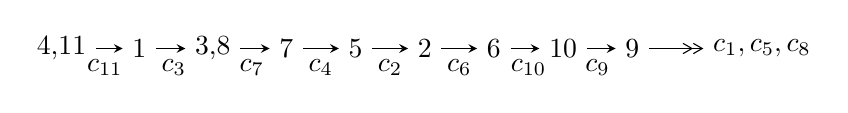
\begin{tikzpicture}[x=25pt, y=7pt]
	% node
	\node (A0) at (-1/8, 0) {4,11};
	\node (A1) at (1, 0) {1};
	\node (A2) at (33/16, 0) {3,8};
	\node (A3) at (25/8, 0) {7};
	\node (A4) at (33/8, 0) {5};
	\node (A5) at (41/8, 0) {2};
	\node (A6) at (49/8, 0) {6};
	\node (A7) at (57/8, 0) {10};
	\node (A8) at (65/8, 0) {9};
	\node (C1) at (1/2, -1) {$c_{11}$};
	\node (C2) at (3/2, -1) {$c_{3}$};
	\node (C3) at (21/8, -1) {$c_{7}$};
	\node (C4) at (29/8, -1) {$c_{4}$};
	\node (C5) at (37/8, -1) {$c_{2}$};
	\node (C6) at (45/8, -1) {$c_{6}$};
	\node (C7) at (53/8, -1) {$c_{10}$};
	\node (C8) at (61/8, -1) {$c_{9}$};
	\node (A9) at (10, 0) {$c_{1},c_{5},c_{8}$};

	% edge
	\draw[->,>=stealth]	
	(A0) edge (A1) (A1) edge (A2) (A2) edge (A3) (A3) edge (A4) (A4) edge (A5) (A5) edge (A6) (A6) edge (A7) (A7) edge (A8) ;
	\draw[->>,>={angle 60}]	
	(A8) edge (A9);
\end{tikzpicture} \\ 

\end{tabular} \\

\footnotetext{
The image of knot diagram is generated by the software ``\textbf{Draw programme}" developed by Andrew Bartholomew(\url{http://www.layer8.co.uk/maths/draw/index.htm\#Running-draw}), where we modified some parts for our purpose(\url{https://github.com/CATsTAILs/LinksPainter}).
}\phantom \\ \newline 
\centering \textbf{Ideals for irreducible components\footnotemark of $X_{\text{par}}$} 
 
\begin{align*}
I^u_{1}&=\langle 
b+u,\;-3 u^{12}-15 u^{11}+\cdots+11 a-20,\\
\phantom{I^u_{1}}&\phantom{= \langle  }u^{13}+u^{12}+7 u^{11}+6 u^{10}+19 u^9+15 u^8+22 u^7+18 u^6+7 u^5+10 u^4+2 u^2+4 u-1\rangle \\
I^u_{2}&=\langle 
-62903946761724 u^{25}-381362114178501 u^{24}+\cdots+640188464864309 b-1417634446440228,\\
\phantom{I^u_{2}}&\phantom{= \langle  }911334568428454 u^{25}+2453993677512419 u^{24}+\cdots+640188464864309 a-843495134320420,\\
\phantom{I^u_{2}}&\phantom{= \langle  }u^{26}+3 u^{25}+\cdots+9 u+1\rangle \\
I^u_{3}&=\langle 
b+u,\;- u^5+u^4-3 u^3+u^2+a-3 u+1,\;u^6- u^5+3 u^4-2 u^3+3 u^2-2 u+1\rangle \\
I^u_{4}&=\langle 
- u^3+u^2+b-2 u+2,\;- u^5+2 u^4- u^3+3 a+3 u-4,\;u^6-2 u^5+4 u^4-6 u^3+6 u^2-5 u+3\rangle \\
\\
\end{align*}
\raggedright * 4 irreducible components of $\dim_{\mathbb{C}}=0$, with total 51 representations.\\
\footnotetext{All coefficients of polynomials are rational numbers. But the coefficients are sometimes approximated in decimal forms when there is not enough margin.}
\newpage
\renewcommand{\arraystretch}{1}
\centering \section*{I. $I^u_{1}= \langle b+u,\;-3 u^{12}-15 u^{11}+\cdots+11 a-20,\;u^{13}+u^{12}+\cdots+4 u-1 \rangle$}
\flushleft \textbf{(i) Arc colorings}\\
\begin{tabular}{m{7pt} m{180pt} m{7pt} m{180pt} }
\flushright $a_{4}=$&$\begin{pmatrix}0\\u\end{pmatrix}$ \\
\flushright $a_{11}=$&$\begin{pmatrix}1\\0\end{pmatrix}$ \\
\flushright $a_{1}=$&$\begin{pmatrix}1\\u^2\end{pmatrix}$ \\
\flushright $a_{3}=$&$\begin{pmatrix}u\\u^3+u\end{pmatrix}$ \\
\flushright $a_{8}=$&$\begin{pmatrix}0.272727 u^{12}+1.36364 u^{11}+\cdots+5.18182 u+1.81818\\- u\end{pmatrix}$ \\
\flushright $a_{7}=$&$\begin{pmatrix}0.272727 u^{12}+1.36364 u^{11}+\cdots+4.18182 u+1.81818\\- u\end{pmatrix}$ \\
\flushright $a_{5}=$&$\begin{pmatrix}-0.545455 u^{12}+2.27273 u^{11}+\cdots+7.63636 u-3.63636\\0.363636 u^{12}-1.18182 u^{11}+\cdots-3.09091 u+1.09091\end{pmatrix}$ \\
\flushright $a_{2}=$&$\begin{pmatrix}4.81818 u^{12}+4.09091 u^{11}+\cdots-4.45455 u+1.45455\\-2.27273 u^{12}-2.36364 u^{11}+\cdots+0.818182 u+0.181818\end{pmatrix}$ \\
\flushright $a_{6}=$&$\begin{pmatrix}0.0909091 u^{12}+0.454545 u^{11}+\cdots+1.72727 u+2.27273\\-0.0909091 u^{12}+0.545455 u^{11}+\cdots-0.727273 u-0.272727\end{pmatrix}$ \\
\flushright $a_{10}=$&$\begin{pmatrix}1.09091 u^{12}+1.45455 u^{11}+\cdots+0.727273 u+1.27273\\- u^2\end{pmatrix}$ \\
\flushright $a_{9}=$&$\begin{pmatrix}1.81818 u^{12}+2.09091 u^{11}+\cdots-0.454545 u+1.45455\\-0.636364 u^{12}-0.181818 u^{11}+\cdots-0.0909091 u+0.0909091\end{pmatrix}$\\ \flushright $a_{9}=$&$\begin{pmatrix}1.81818 u^{12}+2.09091 u^{11}+\cdots-0.454545 u+1.45455\\-0.636364 u^{12}-0.181818 u^{11}+\cdots-0.0909091 u+0.0909091\end{pmatrix}$\\&\end{tabular}
\flushleft \textbf{(ii) Obstruction class $= -1$}\\~\\
\flushleft \textbf{(iii) Cusp Shapes $= -\frac{4}{11} u^{12}-\frac{42}{11} u^{11}-\frac{75}{11} u^{10}-\frac{247}{11} u^9-\frac{294}{11} u^8-\frac{543}{11} u^7-\frac{478}{11} u^6-\frac{433}{11} u^5-23 u^4-\frac{29}{11} u^3-\frac{28}{11} u^2-\frac{32}{11} u-\frac{89}{11}$}\\~\\
\newpage\renewcommand{\arraystretch}{1}
\flushleft \textbf{(iv) u-Polynomials at the component}\newline \\
\begin{tabular}{m{50pt}|m{274pt}}
Crossings & \hspace{64pt}u-Polynomials at each crossing \\
\hline $$\begin{aligned}c_{1}\end{aligned}$$&$\begin{aligned}
&u^{13}+16 u^{12}+\cdots+384 u+32
\end{aligned}$\\
\hline $$\begin{aligned}c_{2},c_{5}\end{aligned}$$&$\begin{aligned}
&u^{13}+12 u^{11}+\cdots+7 u^2+1
\end{aligned}$\\
\hline $$\begin{aligned}c_{3},c_{7},c_{10}\\c_{11}\end{aligned}$$&$\begin{aligned}
&u^{13}- u^{12}+\cdots+4 u+1
\end{aligned}$\\
\hline $$\begin{aligned}c_{4}\end{aligned}$$&$\begin{aligned}
&u^{13}-11 u^{12}+\cdots-40 u+4
\end{aligned}$\\
\hline $$\begin{aligned}c_{6},c_{8}\end{aligned}$$&$\begin{aligned}
&u^{13}- u^{12}+\cdots-11 u+3
\end{aligned}$\\
\hline $$\begin{aligned}c_{9}\end{aligned}$$&$\begin{aligned}
&u^{13}-8 u^{12}+\cdots+6 u+12
\end{aligned}$\\
\hline
\end{tabular}\\~\\
\newpage\renewcommand{\arraystretch}{1}
\flushleft \textbf{(v) Riley Polynomials at the component}\newline \\
\begin{tabular}{m{50pt}|m{274pt}}
Crossings & \hspace{64pt}Riley Polynomials at each crossing \\
\hline $$\begin{aligned}c_{1}\end{aligned}$$&$\begin{aligned}
&y^{13}-12 y^{12}+\cdots+59904 y-1024
\end{aligned}$\\
\hline $$\begin{aligned}c_{2},c_{5}\end{aligned}$$&$\begin{aligned}
&y^{13}+24 y^{12}+\cdots-14 y-1
\end{aligned}$\\
\hline $$\begin{aligned}c_{3},c_{7},c_{10}\\c_{11}\end{aligned}$$&$\begin{aligned}
&y^{13}+13 y^{12}+\cdots+20 y-1
\end{aligned}$\\
\hline $$\begin{aligned}c_{4}\end{aligned}$$&$\begin{aligned}
&y^{13}-3 y^{12}+\cdots+456 y-16
\end{aligned}$\\
\hline $$\begin{aligned}c_{6},c_{8}\end{aligned}$$&$\begin{aligned}
&y^{13}+11 y^{12}+\cdots-35 y-9
\end{aligned}$\\
\hline $$\begin{aligned}c_{9}\end{aligned}$$&$\begin{aligned}
&y^{13}-14 y^{12}+\cdots+732 y-144
\end{aligned}$\\
\hline
\end{tabular}\\~\\
\newpage\flushleft \textbf{(vi) Complex Volumes and Cusp Shapes}
$$\begin{array}{c|c|c}  
\text{Solutions to }I^u_{1}& \I (\text{vol} + \sqrt{-1}CS) & \text{Cusp shape}\\
 \hline 
\begin{aligned}
u &= -0.809423 + 0.117584 I \\
a &= \phantom{-}0.348533 - 0.706548 I \\
b &= \phantom{-}0.809423 - 0.117584 I\end{aligned}
 & \phantom{-}5.36911 + 2.95494 I & -7.16291 - 2.81901 I \\ \hline\begin{aligned}
u &= -0.809423 - 0.117584 I \\
a &= \phantom{-}0.348533 + 0.706548 I \\
b &= \phantom{-}0.809423 + 0.117584 I\end{aligned}
 & \phantom{-}5.36911 - 2.95494 I & -7.16291 + 2.81901 I \\ \hline\begin{aligned}
u &= -0.046196 + 1.261130 I \\
a &= -1.11366 + 3.26926 I \\
b &= \phantom{-}0.046196 - 1.261130 I\end{aligned}
 & \phantom{-}12.31700 + 2.15873 I & \phantom{-}3.13107 - 3.07256 I \\ \hline\begin{aligned}
u &= -0.046196 - 1.261130 I \\
a &= -1.11366 - 3.26926 I \\
b &= \phantom{-}0.046196 + 1.261130 I\end{aligned}
 & \phantom{-}12.31700 - 2.15873 I & \phantom{-}3.13107 + 3.07256 I \\ \hline\begin{aligned}
u &= -0.151527 + 1.292460 I \\
a &= \phantom{-}0.71662 + 1.73016 I \\
b &= \phantom{-}0.151527 - 1.292460 I\end{aligned}
 & \phantom{-}6.35965 - 0.39707 I & -2.26484 + 2.21487 I \\ \hline\begin{aligned}
u &= -0.151527 - 1.292460 I \\
a &= \phantom{-}0.71662 - 1.73016 I \\
b &= \phantom{-}0.151527 + 1.292460 I\end{aligned}
 & \phantom{-}6.35965 + 0.39707 I & -2.26484 - 2.21487 I \\ \hline\begin{aligned}
u &= \phantom{-}0.479303 + 0.472811 I \\
a &= \phantom{-}0.182244 + 0.741863 I \\
b &= -0.479303 - 0.472811 I\end{aligned}
 & -0.52618 - 1.43256 I & -3.73519 + 6.28375 I \\ \hline\begin{aligned}
u &= \phantom{-}0.479303 - 0.472811 I \\
a &= \phantom{-}0.182244 - 0.741863 I \\
b &= -0.479303 + 0.472811 I\end{aligned}
 & -0.52618 + 1.43256 I & -3.73519 - 6.28375 I \\ \hline\begin{aligned}
u &= \phantom{-}0.40436 + 1.44082 I \\
a &= -0.36627 + 1.65681 I \\
b &= -0.40436 - 1.44082 I\end{aligned}
 & \phantom{-}6.52797 - 5.89125 I & -0.30193 + 3.39089 I \\ \hline\begin{aligned}
u &= \phantom{-}0.40436 - 1.44082 I \\
a &= -0.36627 - 1.65681 I \\
b &= -0.40436 + 1.44082 I\end{aligned}
 & \phantom{-}6.52797 + 5.89125 I & -0.30193 - 3.39089 I\\
 \hline 
 \end{array}$$\newpage$$\begin{array}{c|c|c}  
\text{Solutions to }I^u_{1}& \I (\text{vol} + \sqrt{-1}CS) & \text{Cusp shape}\\
 \hline 
\begin{aligned}
u &= -0.48592 + 1.50310 I \\
a &= \phantom{-}0.64061 + 1.74510 I \\
b &= \phantom{-}0.48592 - 1.50310 I\end{aligned}
 & \phantom{-}15.6748 + 13.1069 I & -1.18846 - 5.87531 I \\ \hline\begin{aligned}
u &= -0.48592 - 1.50310 I \\
a &= \phantom{-}0.64061 - 1.74510 I \\
b &= \phantom{-}0.48592 + 1.50310 I\end{aligned}
 & \phantom{-}15.6748 - 13.1069 I & -1.18846 + 5.87531 I \\ \hline\begin{aligned}
u &= \phantom{-}0.218803\phantom{ +0.000000I} \\
a &= \phantom{-}3.18385\phantom{ +0.000000I} \\
b &= -0.218803\phantom{ +0.000000I}\end{aligned}
 & -0.973187\phantom{ +0.000000I} & -8.95550\phantom{ +0.000000I}\\
 \hline 
 \end{array}$$\newpage\newpage\renewcommand{\arraystretch}{1}
\centering \section*{II. $I^u_{2}= \langle -6.29\times10^{13} u^{25}-3.81\times10^{14} u^{24}+\cdots+6.40\times10^{14} b-1.42\times10^{15},\;9.11\times10^{14} u^{25}+2.45\times10^{15} u^{24}+\cdots+6.40\times10^{14} a-8.43\times10^{14},\;u^{26}+3 u^{25}+\cdots+9 u+1 \rangle$}
\flushleft \textbf{(i) Arc colorings}\\
\begin{tabular}{m{7pt} m{180pt} m{7pt} m{180pt} }
\flushright $a_{4}=$&$\begin{pmatrix}0\\u\end{pmatrix}$ \\
\flushright $a_{11}=$&$\begin{pmatrix}1\\0\end{pmatrix}$ \\
\flushright $a_{1}=$&$\begin{pmatrix}1\\u^2\end{pmatrix}$ \\
\flushright $a_{3}=$&$\begin{pmatrix}u\\u^3+u\end{pmatrix}$ \\
\flushright $a_{8}=$&$\begin{pmatrix}-1.42354 u^{25}-3.83324 u^{24}+\cdots-30.3254 u+1.31757\\0.0982585 u^{25}+0.595703 u^{24}+\cdots+12.7692 u+2.21440\end{pmatrix}$ \\
\flushright $a_{7}=$&$\begin{pmatrix}-1.32528 u^{25}-3.23753 u^{24}+\cdots-17.5562 u+3.53197\\0.0982585 u^{25}+0.595703 u^{24}+\cdots+12.7692 u+2.21440\end{pmatrix}$ \\
\flushright $a_{5}=$&$\begin{pmatrix}-3.59109 u^{25}-10.1484 u^{24}+\cdots-88.3953 u-7.10835\\0.279522 u^{25}+0.762410 u^{24}+\cdots+8.19857 u+2.54254\end{pmatrix}$ \\
\flushright $a_{2}=$&$\begin{pmatrix}1.43267 u^{25}+5.14988 u^{24}+\cdots+85.8161 u+25.6973\\1.45570 u^{25}+4.17786 u^{24}+\cdots+43.0260 u+4.92495\end{pmatrix}$ \\
\flushright $a_{6}=$&$\begin{pmatrix}-1.11476 u^{25}-2.66132 u^{24}+\cdots-13.3210 u+4.20145\\0.383189 u^{25}+1.21076 u^{24}+\cdots+17.2921 u+2.93923\end{pmatrix}$ \\
\flushright $a_{10}=$&$\begin{pmatrix}-1.85007 u^{25}-5.49107 u^{24}+\cdots-77.2940 u-14.2016\\-0.692471 u^{25}-1.85702 u^{24}+\cdots-12.8116 u-0.482676\end{pmatrix}$ \\
\flushright $a_{9}=$&$\begin{pmatrix}-1.71634 u^{25}-5.14621 u^{24}+\cdots-73.8523 u-13.9762\\-0.513166 u^{25}-1.32858 u^{24}+\cdots-8.99682 u-0.200919\end{pmatrix}$\\ \flushright $a_{9}=$&$\begin{pmatrix}-1.71634 u^{25}-5.14621 u^{24}+\cdots-73.8523 u-13.9762\\-0.513166 u^{25}-1.32858 u^{24}+\cdots-8.99682 u-0.200919\end{pmatrix}$\\&\end{tabular}
\flushleft \textbf{(ii) Obstruction class $= -1$}\\~\\
\flushleft \textbf{(iii) Cusp Shapes $= \frac{835837455787153}{640188464864309} u^{25}+\frac{1938384712386284}{640188464864309} u^{24}+\cdots+\frac{13509636668298897}{640188464864309} u-\frac{455441820193168}{640188464864309}$}\\~\\
\newpage\renewcommand{\arraystretch}{1}
\flushleft \textbf{(iv) u-Polynomials at the component}\newline \\
\begin{tabular}{m{50pt}|m{274pt}}
Crossings & \hspace{64pt}u-Polynomials at each crossing \\
\hline $$\begin{aligned}c_{1}\end{aligned}$$&$\begin{aligned}
&(u^{13}-4 u^{12}+\cdots+47 u+1)^{2}
\end{aligned}$\\
\hline $$\begin{aligned}c_{2},c_{5}\end{aligned}$$&$\begin{aligned}
&u^{26}- u^{25}+\cdots+193 u+61
\end{aligned}$\\
\hline $$\begin{aligned}c_{3},c_{7},c_{10}\\c_{11}\end{aligned}$$&$\begin{aligned}
&u^{26}-3 u^{25}+\cdots-9 u+1
\end{aligned}$\\
\hline $$\begin{aligned}c_{4}\end{aligned}$$&$\begin{aligned}
&(u^{13}+u^{12}+\cdots+8 u+5)^{2}
\end{aligned}$\\
\hline $$\begin{aligned}c_{6},c_{8}\end{aligned}$$&$\begin{aligned}
&u^{26}+4 u^{25}+\cdots+2400 u+1353
\end{aligned}$\\
\hline $$\begin{aligned}c_{9}\end{aligned}$$&$\begin{aligned}
&(u^{13}+3 u^{12}+\cdots+2 u+3)^{2}
\end{aligned}$\\
\hline
\end{tabular}\\~\\
\newpage\renewcommand{\arraystretch}{1}
\flushleft \textbf{(v) Riley Polynomials at the component}\newline \\
\begin{tabular}{m{50pt}|m{274pt}}
Crossings & \hspace{64pt}Riley Polynomials at each crossing \\
\hline $$\begin{aligned}c_{1}\end{aligned}$$&$\begin{aligned}
&(y^{13}-16 y^{12}+\cdots+2493 y-1)^{2}
\end{aligned}$\\
\hline $$\begin{aligned}c_{2},c_{5}\end{aligned}$$&$\begin{aligned}
&y^{26}+33 y^{25}+\cdots+38147 y+3721
\end{aligned}$\\
\hline $$\begin{aligned}c_{3},c_{7},c_{10}\\c_{11}\end{aligned}$$&$\begin{aligned}
&y^{26}+19 y^{25}+\cdots- y+1
\end{aligned}$\\
\hline $$\begin{aligned}c_{4}\end{aligned}$$&$\begin{aligned}
&(y^{13}+9 y^{12}+\cdots-136 y-25)^{2}
\end{aligned}$\\
\hline $$\begin{aligned}c_{6},c_{8}\end{aligned}$$&$\begin{aligned}
&y^{26}+20 y^{25}+\cdots+9336774 y+1830609
\end{aligned}$\\
\hline $$\begin{aligned}c_{9}\end{aligned}$$&$\begin{aligned}
&(y^{13}-19 y^{12}+\cdots+124 y-9)^{2}
\end{aligned}$\\
\hline
\end{tabular}\\~\\
\newpage\flushleft \textbf{(vi) Complex Volumes and Cusp Shapes}
$$\begin{array}{c|c|c}  
\text{Solutions to }I^u_{2}& \I (\text{vol} + \sqrt{-1}CS) & \text{Cusp shape}\\
 \hline 
\begin{aligned}
u &= \phantom{-}0.067900 + 1.180330 I \\
a &= \phantom{-}0.517992 - 0.149968 I \\
b &= -1.207500 - 0.051879 I\end{aligned}
 & \phantom{-}1.265650 - 0.287296 I & -2.88954 - 0.89161 I \\ \hline\begin{aligned}
u &= \phantom{-}0.067900 - 1.180330 I \\
a &= \phantom{-}0.517992 + 0.149968 I \\
b &= -1.207500 + 0.051879 I\end{aligned}
 & \phantom{-}1.265650 + 0.287296 I & -2.88954 + 0.89161 I \\ \hline\begin{aligned}
u &= \phantom{-}0.247316 + 1.177340 I \\
a &= \phantom{-}0.311935 - 0.046135 I \\
b &= \phantom{-}0.524618 - 0.069053 I\end{aligned}
 & \phantom{-}2.03958 - 2.67289 I & -1.48191 + 5.19592 I \\ \hline\begin{aligned}
u &= \phantom{-}0.247316 - 1.177340 I \\
a &= \phantom{-}0.311935 + 0.046135 I \\
b &= \phantom{-}0.524618 + 0.069053 I\end{aligned}
 & \phantom{-}2.03958 + 2.67289 I & -1.48191 - 5.19592 I \\ \hline\begin{aligned}
u &= \phantom{-}1.207500 + 0.051879 I \\
a &= \phantom{-}0.196751 + 0.489452 I \\
b &= -0.067900 - 1.180330 I\end{aligned}
 & \phantom{-}1.265650 - 0.287296 I & -2.88954 - 0.89161 I \\ \hline\begin{aligned}
u &= \phantom{-}1.207500 - 0.051879 I \\
a &= \phantom{-}0.196751 - 0.489452 I \\
b &= -0.067900 + 1.180330 I\end{aligned}
 & \phantom{-}1.265650 + 0.287296 I & -2.88954 + 0.89161 I \\ \hline\begin{aligned}
u &= -0.216549 + 1.266240 I \\
a &= -0.86731 - 1.86678 I \\
b &= -0.45644 + 1.36303 I\end{aligned}
 & \phantom{-}5.76658 + 5.41588 I & -0.94009 - 2.54727 I \\ \hline\begin{aligned}
u &= -0.216549 - 1.266240 I \\
a &= -0.86731 + 1.86678 I \\
b &= -0.45644 - 1.36303 I\end{aligned}
 & \phantom{-}5.76658 - 5.41588 I & -0.94009 + 2.54727 I \\ \hline\begin{aligned}
u &= -1.274900 + 0.275508 I \\
a &= \phantom{-}0.251587 + 0.623600 I \\
b &= \phantom{-}0.326804 - 1.347110 I\end{aligned}
 & \phantom{-}10.00280 + 7.01304 I & -2.38090 - 4.98186 I \\ \hline\begin{aligned}
u &= -1.274900 - 0.275508 I \\
a &= \phantom{-}0.251587 - 0.623600 I \\
b &= \phantom{-}0.326804 + 1.347110 I\end{aligned}
 & \phantom{-}10.00280 - 7.01304 I & -2.38090 + 4.98186 I\\
 \hline 
 \end{array}$$\newpage$$\begin{array}{c|c|c}  
\text{Solutions to }I^u_{2}& \I (\text{vol} + \sqrt{-1}CS) & \text{Cusp shape}\\
 \hline 
\begin{aligned}
u &= -0.394224 + 1.245000 I \\
a &= -0.638079 + 0.785356 I \\
b &= \phantom{-}0.160428 + 0.147487 I\end{aligned}
 & \phantom{-}8.78740 + 1.45996 I & -3.65650 - 0.27682 I \\ \hline\begin{aligned}
u &= -0.394224 - 1.245000 I \\
a &= -0.638079 - 0.785356 I \\
b &= \phantom{-}0.160428 - 0.147487 I\end{aligned}
 & \phantom{-}8.78740 - 1.45996 I & -3.65650 + 0.27682 I \\ \hline\begin{aligned}
u &= -0.052461 + 1.357580 I \\
a &= -0.07916 - 1.70109 I \\
b &= \phantom{-}0.78161 + 1.55425 I\end{aligned}
 & \phantom{-}13.70610 - 0.67900 I & \phantom{-}1.58151 + 0.47574 I \\ \hline\begin{aligned}
u &= -0.052461 - 1.357580 I \\
a &= -0.07916 + 1.70109 I \\
b &= \phantom{-}0.78161 - 1.55425 I\end{aligned}
 & \phantom{-}13.70610 + 0.67900 I & \phantom{-}1.58151 - 0.47574 I \\ \hline\begin{aligned}
u &= -0.326804 + 1.347110 I \\
a &= -0.425005 + 0.468743 I \\
b &= \phantom{-}1.274900 - 0.275508 I\end{aligned}
 & \phantom{-}10.00280 + 7.01304 I & -2.38090 - 4.98186 I \\ \hline\begin{aligned}
u &= -0.326804 - 1.347110 I \\
a &= -0.425005 - 0.468743 I \\
b &= \phantom{-}1.274900 + 0.275508 I\end{aligned}
 & \phantom{-}10.00280 - 7.01304 I & -2.38090 + 4.98186 I \\ \hline\begin{aligned}
u &= \phantom{-}0.45644 + 1.36303 I \\
a &= \phantom{-}1.02148 - 1.52994 I \\
b &= \phantom{-}0.216549 + 1.266240 I\end{aligned}
 & \phantom{-}5.76658 - 5.41588 I & -0.94009 + 2.54727 I \\ \hline\begin{aligned}
u &= \phantom{-}0.45644 - 1.36303 I \\
a &= \phantom{-}1.02148 + 1.52994 I \\
b &= \phantom{-}0.216549 - 1.266240 I\end{aligned}
 & \phantom{-}5.76658 + 5.41588 I & -0.94009 - 2.54727 I \\ \hline\begin{aligned}
u &= -0.524618 + 0.069053 I \\
a &= -0.158561 - 0.699160 I \\
b &= -0.247316 - 1.177340 I\end{aligned}
 & \phantom{-}2.03958 - 2.67289 I & -1.48191 + 5.19592 I \\ \hline\begin{aligned}
u &= -0.524618 - 0.069053 I \\
a &= -0.158561 + 0.699160 I \\
b &= -0.247316 + 1.177340 I\end{aligned}
 & \phantom{-}2.03958 + 2.67289 I & -1.48191 - 5.19592 I\\
 \hline 
 \end{array}$$\newpage$$\begin{array}{c|c|c}  
\text{Solutions to }I^u_{2}& \I (\text{vol} + \sqrt{-1}CS) & \text{Cusp shape}\\
 \hline 
\begin{aligned}
u &= \phantom{-}0.252433 + 0.419434 I \\
a &= \phantom{-}1.07447 - 1.78530 I \\
b &= -0.252433 + 0.419434 I\end{aligned}
 & -0.889471\phantom{ +0.000000I} & -5.46516 + 0. I\phantom{ +0.000000I} \\ \hline\begin{aligned}
u &= \phantom{-}0.252433 - 0.419434 I \\
a &= \phantom{-}1.07447 + 1.78530 I \\
b &= -0.252433 - 0.419434 I\end{aligned}
 & -0.889471\phantom{ +0.000000I} & -5.46516 + 0. I\phantom{ +0.000000I} \\ \hline\begin{aligned}
u &= -0.78161 + 1.55425 I \\
a &= -0.588096 - 1.192760 I \\
b &= \phantom{-}0.052461 + 1.357580 I\end{aligned}
 & \phantom{-}13.70610 + 0.67900 I & \phantom{-}1.58151 + 0. I\phantom{ +0.000000I} \\ \hline\begin{aligned}
u &= -0.78161 - 1.55425 I \\
a &= -0.588096 + 1.192760 I \\
b &= \phantom{-}0.052461 - 1.357580 I\end{aligned}
 & \phantom{-}13.70610 - 0.67900 I & \phantom{-}1.58151 + 0. I\phantom{ +0.000000I} \\ \hline\begin{aligned}
u &= -0.160428 + 0.147487 I \\
a &= \phantom{-}5.88200 - 1.47414 I \\
b &= \phantom{-}0.394224 + 1.245000 I\end{aligned}
 & \phantom{-}8.78740 - 1.45996 I & -3.65650 + 0.27682 I \\ \hline\begin{aligned}
u &= -0.160428 - 0.147487 I \\
a &= \phantom{-}5.88200 + 1.47414 I \\
b &= \phantom{-}0.394224 - 1.245000 I\end{aligned}
 & \phantom{-}8.78740 + 1.45996 I & -3.65650 - 0.27682 I\\
 \hline 
 \end{array}$$\newpage\newpage\renewcommand{\arraystretch}{1}
\centering \section*{III. $I^u_{3}= \langle b+u,\;- u^5+u^4-3 u^3+u^2+a-3 u+1,\;u^6- u^5+3 u^4-2 u^3+3 u^2-2 u+1 \rangle$}
\flushleft \textbf{(i) Arc colorings}\\
\begin{tabular}{m{7pt} m{180pt} m{7pt} m{180pt} }
\flushright $a_{4}=$&$\begin{pmatrix}0\\u\end{pmatrix}$ \\
\flushright $a_{11}=$&$\begin{pmatrix}1\\0\end{pmatrix}$ \\
\flushright $a_{1}=$&$\begin{pmatrix}1\\u^2\end{pmatrix}$ \\
\flushright $a_{3}=$&$\begin{pmatrix}u\\u^3+u\end{pmatrix}$ \\
\flushright $a_{8}=$&$\begin{pmatrix}u^5- u^4+3 u^3- u^2+3 u-1\\- u\end{pmatrix}$ \\
\flushright $a_{7}=$&$\begin{pmatrix}u^5- u^4+3 u^3- u^2+2 u-1\\- u\end{pmatrix}$ \\
\flushright $a_{5}=$&$\begin{pmatrix}u^4+2 u^2\\u^4- u^3+u^2\end{pmatrix}$ \\
\flushright $a_{2}=$&$\begin{pmatrix}u^2- u+1\\u^5+u^3+2 u^2- u+1\end{pmatrix}$ \\
\flushright $a_{6}=$&$\begin{pmatrix}u^5+2 u^3+u^2+u\\0\end{pmatrix}$ \\
\flushright $a_{10}=$&$\begin{pmatrix}u^3+u\\- u^2\end{pmatrix}$ \\
\flushright $a_{9}=$&$\begin{pmatrix}u^3- u^2+2 u-1\\- u^4+u^3-3 u^2+u-1\end{pmatrix}$\\ \flushright $a_{9}=$&$\begin{pmatrix}u^3- u^2+2 u-1\\- u^4+u^3-3 u^2+u-1\end{pmatrix}$\\&\end{tabular}
\flushleft \textbf{(ii) Obstruction class $= 1$}\\~\\
\flushleft \textbf{(iii) Cusp Shapes $= 7 u^5-9 u^4+19 u^3-13 u^2+14 u-15$}\\~\\
\newpage\renewcommand{\arraystretch}{1}
\flushleft \textbf{(iv) u-Polynomials at the component}\newline \\
\begin{tabular}{m{50pt}|m{274pt}}
Crossings & \hspace{64pt}u-Polynomials at each crossing \\
\hline $$\begin{aligned}c_{1}\end{aligned}$$&$\begin{aligned}
&u^6- u^5+8 u^3+3 u^2- u+3
\end{aligned}$\\
\hline $$\begin{aligned}c_{2},c_{5}\end{aligned}$$&$\begin{aligned}
&u^6+2 u^4+3 u^3-2 u^2-2 u+1
\end{aligned}$\\
\hline $$\begin{aligned}c_{3},c_{10}\end{aligned}$$&$\begin{aligned}
&u^6+u^5+3 u^4+2 u^3+3 u^2+2 u+1
\end{aligned}$\\
\hline $$\begin{aligned}c_{4}\end{aligned}$$&$\begin{aligned}
&u^6-2 u^5+3 u^4-2 u^3+5 u^2-7 u+3
\end{aligned}$\\
\hline $$\begin{aligned}c_{6},c_{8}\end{aligned}$$&$\begin{aligned}
&u^6+u^5+2 u^4+2 u^3+u^2+u+1
\end{aligned}$\\
\hline $$\begin{aligned}c_{7},c_{11}\end{aligned}$$&$\begin{aligned}
&u^6- u^5+3 u^4-2 u^3+3 u^2-2 u+1
\end{aligned}$\\
\hline $$\begin{aligned}c_{9}\end{aligned}$$&$\begin{aligned}
&u^6-3 u^5+2 u^4+u^2- u+1
\end{aligned}$\\
\hline
\end{tabular}\\~\\
\newpage\renewcommand{\arraystretch}{1}
\flushleft \textbf{(v) Riley Polynomials at the component}\newline \\
\begin{tabular}{m{50pt}|m{274pt}}
Crossings & \hspace{64pt}Riley Polynomials at each crossing \\
\hline $$\begin{aligned}c_{1}\end{aligned}$$&$\begin{aligned}
&y^6- y^5+22 y^4-60 y^3+25 y^2+17 y+9
\end{aligned}$\\
\hline $$\begin{aligned}c_{2},c_{5}\end{aligned}$$&$\begin{aligned}
&y^6+4 y^5-15 y^3+20 y^2-8 y+1
\end{aligned}$\\
\hline $$\begin{aligned}c_{3},c_{7},c_{10}\\c_{11}\end{aligned}$$&$\begin{aligned}
&y^6+5 y^5+11 y^4+12 y^3+7 y^2+2 y+1
\end{aligned}$\\
\hline $$\begin{aligned}c_{4}\end{aligned}$$&$\begin{aligned}
&y^6+2 y^5+11 y^4+4 y^3+15 y^2-19 y+9
\end{aligned}$\\
\hline $$\begin{aligned}c_{6},c_{8}\end{aligned}$$&$\begin{aligned}
&y^6+3 y^5+2 y^4+y^2+y+1
\end{aligned}$\\
\hline $$\begin{aligned}c_{9}\end{aligned}$$&$\begin{aligned}
&y^6-5 y^5+6 y^4+5 y^2+y+1
\end{aligned}$\\
\hline
\end{tabular}\\~\\
\newpage\flushleft \textbf{(vi) Complex Volumes and Cusp Shapes}
$$\begin{array}{c|c|c}  
\text{Solutions to }I^u_{3}& \I (\text{vol} + \sqrt{-1}CS) & \text{Cusp shape}\\
 \hline 
\begin{aligned}
u &= -0.368622 + 1.044700 I \\
a &= \phantom{-}0.344849 + 0.081037 I \\
b &= \phantom{-}0.368622 - 1.044700 I\end{aligned}
 & \phantom{-}9.91965 + 2.91185 I & -0.22592 - 3.63955 I \\ \hline\begin{aligned}
u &= -0.368622 - 1.044700 I \\
a &= \phantom{-}0.344849 - 0.081037 I \\
b &= \phantom{-}0.368622 + 1.044700 I\end{aligned}
 & \phantom{-}9.91965 - 2.91185 I & -0.22592 + 3.63955 I \\ \hline\begin{aligned}
u &= \phantom{-}0.474902 + 0.458521 I \\
a &= -0.07450 + 1.48771 I \\
b &= -0.474902 - 0.458521 I\end{aligned}
 & -1.33814 - 0.90202 I & -11.17385 + 4.13696 I \\ \hline\begin{aligned}
u &= \phantom{-}0.474902 - 0.458521 I \\
a &= -0.07450 - 1.48771 I \\
b &= -0.474902 + 0.458521 I\end{aligned}
 & -1.33814 + 0.90202 I & -11.17385 - 4.13696 I \\ \hline\begin{aligned}
u &= \phantom{-}0.393720 + 1.309500 I \\
a &= -0.77035 + 1.73149 I \\
b &= -0.393720 - 1.309500 I\end{aligned}
 & \phantom{-}4.57797 - 6.62522 I & -5.60023 + 6.47362 I \\ \hline\begin{aligned}
u &= \phantom{-}0.393720 - 1.309500 I \\
a &= -0.77035 - 1.73149 I \\
b &= -0.393720 + 1.309500 I\end{aligned}
 & \phantom{-}4.57797 + 6.62522 I & -5.60023 - 6.47362 I\\
 \hline 
 \end{array}$$\newpage\newpage\renewcommand{\arraystretch}{1}
\centering \section*{IV. $I^u_{4}= \langle - u^3+u^2+b-2 u+2,\;- u^5+2 u^4- u^3+3 a+3 u-4,\;u^6-2 u^5+4 u^4-6 u^3+6 u^2-5 u+3 \rangle$}
\flushleft \textbf{(i) Arc colorings}\\
\begin{tabular}{m{7pt} m{180pt} m{7pt} m{180pt} }
\flushright $a_{4}=$&$\begin{pmatrix}0\\u\end{pmatrix}$ \\
\flushright $a_{11}=$&$\begin{pmatrix}1\\0\end{pmatrix}$ \\
\flushright $a_{1}=$&$\begin{pmatrix}1\\u^2\end{pmatrix}$ \\
\flushright $a_{3}=$&$\begin{pmatrix}u\\u^3+u\end{pmatrix}$ \\
\flushright $a_{8}=$&$\begin{pmatrix}\frac{1}{3} u^5-\frac{2}{3} u^4+\frac{1}{3} u^3- u+\frac{4}{3}\\u^3- u^2+2 u-2\end{pmatrix}$ \\
\flushright $a_{7}=$&$\begin{pmatrix}\frac{1}{3} u^5-\frac{2}{3} u^4+\cdots+u-\frac{2}{3}\\u^3- u^2+2 u-2\end{pmatrix}$ \\
\flushright $a_{5}=$&$\begin{pmatrix}-\frac{2}{3} u^5+\frac{4}{3} u^4+\cdots- u+\frac{1}{3}\\u^2+1\end{pmatrix}$ \\
\flushright $a_{2}=$&$\begin{pmatrix}-\frac{1}{3} u^5+\frac{5}{3} u^4+\cdots-3 u+\frac{5}{3}\\- u^4+2 u^3-2 u^2+2 u-1\end{pmatrix}$ \\
\flushright $a_{6}=$&$\begin{pmatrix}\frac{1}{3} u^5+\frac{1}{3} u^4+\cdots-3 u+\frac{7}{3}\\u^3- u^2+3 u-2\end{pmatrix}$ \\
\flushright $a_{10}=$&$\begin{pmatrix}-\frac{1}{3} u^5+\frac{5}{3} u^4+\cdots-4 u+\frac{8}{3}\\- u^4+2 u^3-2 u^2+3 u-1\end{pmatrix}$ \\
\flushright $a_{9}=$&$\begin{pmatrix}-\frac{1}{3} u^5+\frac{2}{3} u^4+\cdots-3 u+\frac{8}{3}\\- u^5+u^4-2 u^3+3 u^2- u+2\end{pmatrix}$\\ \flushright $a_{9}=$&$\begin{pmatrix}-\frac{1}{3} u^5+\frac{2}{3} u^4+\cdots-3 u+\frac{8}{3}\\- u^5+u^4-2 u^3+3 u^2- u+2\end{pmatrix}$\\&\end{tabular}
\flushleft \textbf{(ii) Obstruction class $= 1$}\\~\\
\flushleft \textbf{(iii) Cusp Shapes $= -3 u^4+3 u^3-6 u^2+6 u-6$}\\~\\
\newpage\renewcommand{\arraystretch}{1}
\flushleft \textbf{(iv) u-Polynomials at the component}\newline \\
\begin{tabular}{m{50pt}|m{274pt}}
Crossings & \hspace{64pt}u-Polynomials at each crossing \\
\hline $$\begin{aligned}c_{1}\end{aligned}$$&$\begin{aligned}
&(u^3+u^2-2 u+1)^2
\end{aligned}$\\
\hline $$\begin{aligned}c_{2},c_{5}\end{aligned}$$&$\begin{aligned}
&u^6+3 u^4-3 u^3- u+3
\end{aligned}$\\
\hline $$\begin{aligned}c_{3},c_{10}\end{aligned}$$&$\begin{aligned}
&u^6+2 u^5+4 u^4+6 u^3+6 u^2+5 u+3
\end{aligned}$\\
\hline $$\begin{aligned}c_{4},c_{9}\end{aligned}$$&$\begin{aligned}
&(u^3+u^2+1)^2
\end{aligned}$\\
\hline $$\begin{aligned}c_{6},c_{8}\end{aligned}$$&$\begin{aligned}
&u^6-3 u^5+5 u^4-2 u^3- u^2+2 u+1
\end{aligned}$\\
\hline $$\begin{aligned}c_{7},c_{11}\end{aligned}$$&$\begin{aligned}
&u^6-2 u^5+4 u^4-6 u^3+6 u^2-5 u+3
\end{aligned}$\\
\hline
\end{tabular}\\~\\
\newpage\renewcommand{\arraystretch}{1}
\flushleft \textbf{(v) Riley Polynomials at the component}\newline \\
\begin{tabular}{m{50pt}|m{274pt}}
Crossings & \hspace{64pt}Riley Polynomials at each crossing \\
\hline $$\begin{aligned}c_{1}\end{aligned}$$&$\begin{aligned}
&(y^3-5 y^2+2 y-1)^2
\end{aligned}$\\
\hline $$\begin{aligned}c_{2},c_{5}\end{aligned}$$&$\begin{aligned}
&y^6+6 y^5+9 y^4-3 y^3+12 y^2- y+9
\end{aligned}$\\
\hline $$\begin{aligned}c_{3},c_{7},c_{10}\\c_{11}\end{aligned}$$&$\begin{aligned}
&y^6+4 y^5+4 y^4-2 y^3+11 y+9
\end{aligned}$\\
\hline $$\begin{aligned}c_{4},c_{9}\end{aligned}$$&$\begin{aligned}
&(y^3- y^2-2 y-1)^2
\end{aligned}$\\
\hline $$\begin{aligned}c_{6},c_{8}\end{aligned}$$&$\begin{aligned}
&y^6+y^5+11 y^4+19 y^2-6 y+1
\end{aligned}$\\
\hline
\end{tabular}\\~\\
\newpage\flushleft \textbf{(vi) Complex Volumes and Cusp Shapes}
$$\begin{array}{c|c|c}  
\text{Solutions to }I^u_{4}& \I (\text{vol} + \sqrt{-1}CS) & \text{Cusp shape}\\
 \hline 
\begin{aligned}
u &= \phantom{-}1.044140 + 0.390425 I \\
a &= \phantom{-}0.242056 - 0.443900 I \\
b &= -0.188646 + 1.182980 I\end{aligned}
 & \phantom{-}1.07850 + 1.58317 I & -4.02349 - 3.48462 I \\ \hline\begin{aligned}
u &= \phantom{-}1.044140 - 0.390425 I \\
a &= \phantom{-}0.242056 + 0.443900 I \\
b &= -0.188646 - 1.182980 I\end{aligned}
 & \phantom{-}1.07850 - 1.58317 I & -4.02349 + 3.48462 I \\ \hline\begin{aligned}
u &= \phantom{-}0.188646 + 1.182980 I \\
a &= \phantom{-}0.360189 - 0.302713 I \\
b &= -1.044140 + 0.390425 I\end{aligned}
 & \phantom{-}1.07850 - 1.58317 I & -4.02349 + 3.48462 I \\ \hline\begin{aligned}
u &= \phantom{-}0.188646 - 1.182980 I \\
a &= \phantom{-}0.360189 + 0.302713 I \\
b &= -1.044140 - 0.390425 I\end{aligned}
 & \phantom{-}1.07850 + 1.58317 I & -4.02349 - 3.48462 I \\ \hline\begin{aligned}
u &= -0.232786 + 1.275990 I \\
a &= -0.43558 - 2.38757 I \\
b &= \phantom{-}0.232786 + 1.275990 I\end{aligned}
 & \phantom{-}11.0025\phantom{ +0.000000I} &                  -6
-0.953017 + 0. 10   I\phantom{ +0.000000I} \\ \hline\begin{aligned}
u &= -0.232786 - 1.275990 I \\
a &= -0.43558 + 2.38757 I \\
b &= \phantom{-}0.232786 - 1.275990 I\end{aligned}
 & \phantom{-}11.0025\phantom{ +0.000000I} &                  -6
-0.953017 + 0. 10   I\phantom{ +0.000000I}\\
 \hline 
 \end{array}$$\newpage
\newpage\renewcommand{\arraystretch}{1}
\centering \section*{ V. u-Polynomials}
\begin{tabular}{m{50pt}|m{274pt}}
Crossings & \hspace{64pt}u-Polynomials at each crossing \\
\hline $$\begin{aligned}c_{1}\end{aligned}$$&$\begin{aligned}
&(u^3+u^2-2 u+1)^2(u^6- u^5+8 u^3+3 u^2- u+3)\\
&\cdot((u^{13}-4 u^{12}+\cdots+47 u+1)^{2})(u^{13}+16 u^{12}+\cdots+384 u+32)
\end{aligned}$\\
\hline $$\begin{aligned}c_{2},c_{5}\end{aligned}$$&$\begin{aligned}
&(u^6+2 u^4+3 u^3-2 u^2-2 u+1)(u^6+3 u^4-3 u^3- u+3)\\
&\cdot(u^{13}+12 u^{11}+\cdots+7 u^2+1)(u^{26}- u^{25}+\cdots+193 u+61)
\end{aligned}$\\
\hline $$\begin{aligned}c_{3},c_{10}\end{aligned}$$&$\begin{aligned}
&(u^6+u^5+3 u^4+2 u^3+3 u^2+2 u+1)\\
&\cdot(u^6+2 u^5+\cdots+5 u+3)(u^{13}- u^{12}+\cdots+4 u+1)\\
&\cdot(u^{26}-3 u^{25}+\cdots-9 u+1)
\end{aligned}$\\
\hline $$\begin{aligned}c_{4}\end{aligned}$$&$\begin{aligned}
&(u^3+u^2+1)^2(u^6-2 u^5+3 u^4-2 u^3+5 u^2-7 u+3)\\
&\cdot(u^{13}-11 u^{12}+\cdots-40 u+4)(u^{13}+u^{12}+\cdots+8 u+5)^{2}
\end{aligned}$\\
\hline $$\begin{aligned}c_{6},c_{8}\end{aligned}$$&$\begin{aligned}
&(u^6-3 u^5+5 u^4-2 u^3- u^2+2 u+1)(u^6+u^5+2 u^4+2 u^3+u^2+u+1)\\
&\cdot(u^{13}- u^{12}+\cdots-11 u+3)(u^{26}+4 u^{25}+\cdots+2400 u+1353)
\end{aligned}$\\
\hline $$\begin{aligned}c_{7},c_{11}\end{aligned}$$&$\begin{aligned}
&(u^6-2 u^5+4 u^4-6 u^3+6 u^2-5 u+3)\\
&\cdot(u^6- u^5+3 u^4-2 u^3+3 u^2-2 u+1)(u^{13}- u^{12}+\cdots+4 u+1)\\
&\cdot(u^{26}-3 u^{25}+\cdots-9 u+1)
\end{aligned}$\\
\hline $$\begin{aligned}c_{9}\end{aligned}$$&$\begin{aligned}
&((u^3+u^2+1)^2)(u^6-3 u^5+\cdots- u+1)(u^{13}-8 u^{12}+\cdots+6 u+12)\\
&\cdot(u^{13}+3 u^{12}+\cdots+2 u+3)^{2}
\end{aligned}$\\
\hline
\end{tabular}\newpage\renewcommand{\arraystretch}{1}
\centering \section*{ VI. Riley Polynomials}
\begin{tabular}{m{50pt}|m{274pt}}
Crossings & \hspace{64pt}Riley Polynomials at each crossing \\
\hline $$\begin{aligned}c_{1}\end{aligned}$$&$\begin{aligned}
&(y^3-5 y^2+2 y-1)^2(y^6- y^5+22 y^4-60 y^3+25 y^2+17 y+9)\\
&\cdot(y^{13}-16 y^{12}+\cdots+2493 y-1)^{2}\\
&\cdot(y^{13}-12 y^{12}+\cdots+59904 y-1024)
\end{aligned}$\\
\hline $$\begin{aligned}c_{2},c_{5}\end{aligned}$$&$\begin{aligned}
&(y^6+4 y^5-15 y^3+20 y^2-8 y+1)(y^6+6 y^5+\cdots- y+9)\\
&\cdot(y^{13}+24 y^{12}+\cdots-14 y-1)(y^{26}+33 y^{25}+\cdots+38147 y+3721)
\end{aligned}$\\
\hline $$\begin{aligned}c_{3},c_{7},c_{10}\\c_{11}\end{aligned}$$&$\begin{aligned}
&(y^6+4 y^5+4 y^4-2 y^3+11 y+9)(y^6+5 y^5+\cdots+2 y+1)\\
&\cdot(y^{13}+13 y^{12}+\cdots+20 y-1)(y^{26}+19 y^{25}+\cdots- y+1)
\end{aligned}$\\
\hline $$\begin{aligned}c_{4}\end{aligned}$$&$\begin{aligned}
&(y^3- y^2-2 y-1)^2(y^6+2 y^5+11 y^4+4 y^3+15 y^2-19 y+9)\\
&\cdot(y^{13}-3 y^{12}+\cdots+456 y-16)(y^{13}+9 y^{12}+\cdots-136 y-25)^{2}
\end{aligned}$\\
\hline $$\begin{aligned}c_{6},c_{8}\end{aligned}$$&$\begin{aligned}
&(y^6+y^5+11 y^4+19 y^2-6 y+1)(y^6+3 y^5+2 y^4+y^2+y+1)\\
&\cdot(y^{13}+11 y^{12}+\cdots-35 y-9)\\
&\cdot(y^{26}+20 y^{25}+\cdots+9336774 y+1830609)
\end{aligned}$\\
\hline $$\begin{aligned}c_{9}\end{aligned}$$&$\begin{aligned}
&(y^3- y^2-2 y-1)^2(y^6-5 y^5+6 y^4+5 y^2+y+1)\\
&\cdot((y^{13}-19 y^{12}+\cdots+124 y-9)^{2})(y^{13}-14 y^{12}+\cdots+732 y-144)
\end{aligned}$\\
\hline
\end{tabular}
\vskip 2pc
\end{document}